\section{NPC Problems}
\subsection{3SAT-Cook-Levin Theorem}
\begin{frame}
    \frametitle{NPC maps}
    \begin{figure}[H]
        \centering
        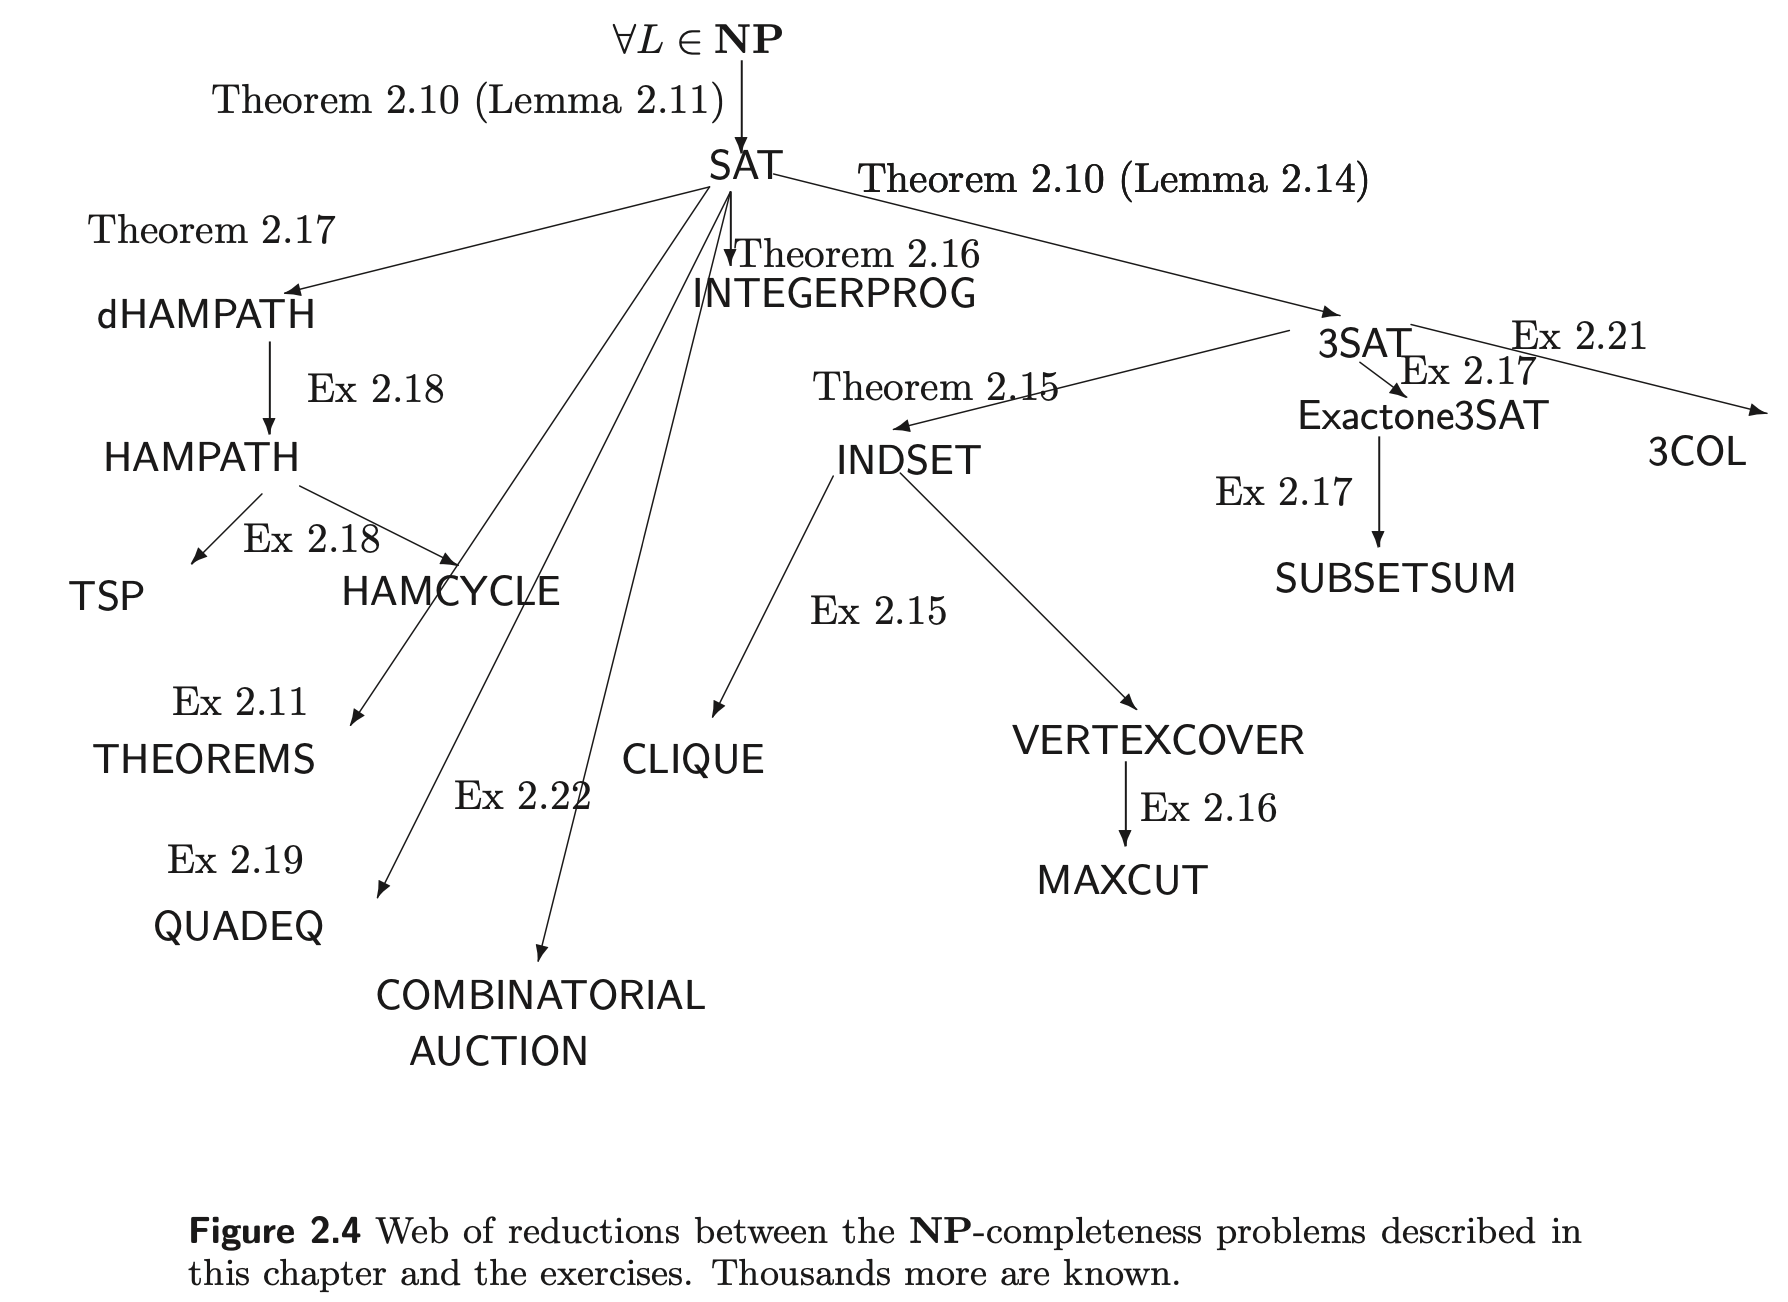
\includegraphics[width=0.95\textwidth]{images/a.png}
        \caption{Another NPC maps}
    \end{figure}
\end{frame}
\begin{frame}
    \frametitle{Definition}
    \begin{definition}[析取范式(CNF)]
        一个布尔表达式$\varphi$, 称$\varphi$为析取范式(CNF), 如果$\varphi$形如:
        \begin{align*}
            \bigwedge_i\left(\bigvee_j v_{i,j}\right)
        \end{align*}
        称$v_{i,j}$为$\varphi$的变量(literal), $(\bigvee_j v_{i,j})$是一个子句(clause).
    \end{definition}
    \pause
    \begin{definition}[SAT and 3SAT]
        $\text{SAT} = \{\text{all satisfiable CNF formulas}\}$ \\
        $\text{3SAT} = \{\text{all satisfiable 3CNF formulas}\}$.
    \end{definition}
\end{frame}
\begin{frame}
    \frametitle{Cook-Levin Theorem}
    \begin{theorem}[Cook-Levin Theorem]
        $\text{3SAT}$是NP-complete的.
    \end{theorem}
    证明: (1) SAT $\in$ NP 是显然的, 考虑证书为一组赋值即可, 验证机只需验证是否可满足.

    (2) SAT 是 NP-hard的. 这个比较困难. 不加证明的给出一个引理.
    \begin{lemma}
        对任意一个布尔函数$f:\{0,1\}^n \rightarrow \{0,1\}$, 可以在$\Theta(2^n)$的时间内构造一个CNF $F$, 使得$f(x) = 1 \iff F(x) = 1$.
    \end{lemma} 
\end{frame}

\subsection{More NPC Problems}
\begin{frame}
    \frametitle{3SAT}
    SAT $\le_p$ 3SAT.
\begin{itemize}
    \item 设$\varphi$是一个CNF公式, 考虑如下规约$f$.
    \item 例如: $(a_1\lor a_2 \lor a_3 \lor a_4) \rightarrow (a_1\lor a_2 \lor z) \land (\bar{z}\lor a_3 \lor a_4)$ 
    \item 一般情况下, 考虑一个有$l$个lieral的子句$(a_1\lor a_2 \lor \cdots \lor a_l)$:
    \begin{align*}
        (a_1\lor a_2 \lor z_1) \land (\bar{z}_1\lor a_3 \lor z_2) \land \cdots \land (\bar{z}_{l-3}\lor a_{l-1}\lor a_l)
    \end{align*}
    总共$l-2$个子句.
\end{itemize}
\end{frame}
\begin{frame}
    \frametitle{MAX-SAT}
    \begin{definition}[MAX-SAT]
        给定一个CNF公式$\varphi$($n$个变量和$m$个子句)和正整数$k$, 如果存在赋值使得$\varphi$中至少有$k$个子句为真, 则$\left\langle \varphi,k\right\rangle \in $MAX-SAT.
    \end{definition}
    SAT $\le_p$ MAX-SAT.
    \begin{itemize}
        \item $\forall \varphi \in$ SAT, 令$k = m$, 则$\left\langle \varphi,k\right\rangle \in$ MAX-SAT.
    \end{itemize}
    MAX-SAT $\in$ NP. 考虑证书为一组赋值即可.
\end{frame}

\begin{frame}
    \frametitle{INDSET}
    \begin{definition}[INDSET]
        给定一个图$G$和正整数$k$, 判定是否存在一个大小为$k$的独立集.
    \end{definition}
    3SAT $\le_p$ INDSET.
    \begin{itemize}
        \item 设$\varphi$是一个3CNF公式(存在$n$个变量和$m$个子句), 构造一个图$G = (V,E)$如下:
        \item $V$: 每个子句$C_i$对于七个点. 这七个点对应7种可能的赋值情况.
        \item $E$: 对应的赋值情况发生冲突, 则在这两点间连边.
    \end{itemize}
\end{frame}

\begin{frame}
    \frametitle{Vertex Cover and CLIQUE}
    \begin{definition}
        \begin{itemize}
            \item \textbf{Vertex Cover}: 给定一个图$G$和正整数$k$, 判定是否存在一个大小不超过$k$的顶点覆盖.
            \item \textbf{CLIQUE}: 给定一个图$G$和正整数$k$, 判定是否存在一个大小不小于$k$的团.
        \end{itemize}
    \end{definition}
    有如下的引理:
    \begin{lemma}
        对任意的无向图$G = (V,E)$和子集$V' \subseteq V$, 下列命题等价:
        \begin{itemize}
            \item $V'$ 是$G$的一个顶点覆盖.
            \item $V-V'$ 是$G$的独立集.
            \item $V - V'$是补图$G_c = (V, E_C)$的团.
        \end{itemize}
    \end{lemma}
\end{frame}

\begin{frame}
    \frametitle{Vertex Cover and CLIQUE(Cont.)}
    INDSET $\le_P$ Vertex Cover.
    \begin{itemize}
        \item $f: \left\langle G,k\right\rangle \rightarrow \left\langle G',k'\right\rangle$, 令$G' = G$, $k' = |V| - k$.
    \end{itemize}
    INDSET $\le_P$ CLIQUE.
    \begin{itemize}
        \item $f: \left\langle G,k\right\rangle \rightarrow \left\langle G',k'\right\rangle $, 令$G' = G_c$, $k' = |V| - k$.
    \end{itemize}
    \begin{figure}
        \centering
        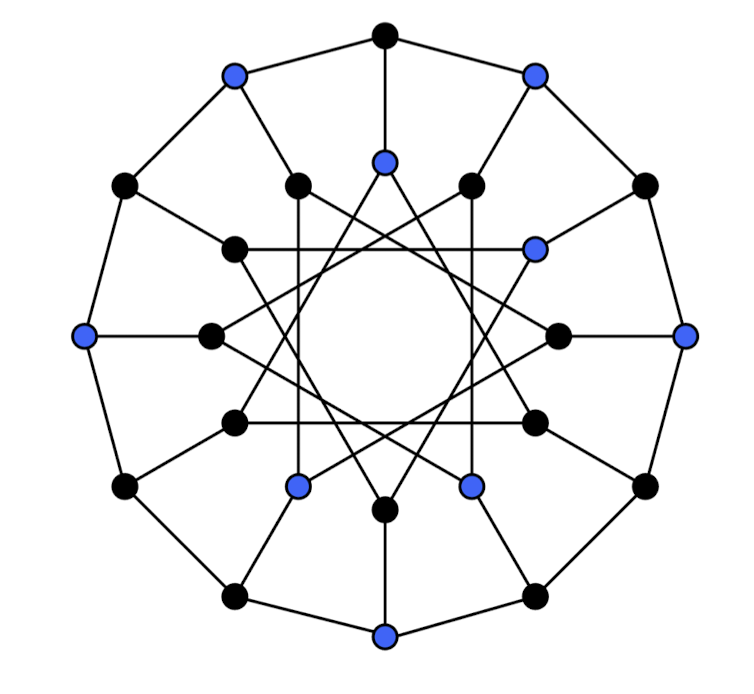
\includegraphics[width=0.5\textwidth]{images/vc.png}
        \caption{Vertex Cover and CLIQUE}
    \end{figure}
\end{frame}

\begin{frame}
    \frametitle{HAMILTONIAN相关问题}
    \begin{definition}
        \begin{itemize}
            \item \textbf{dHAMPATH}: 有向图版本的哈密顿路径.
            \item \textbf{dHAMCYCLE}: 有向图版本的哈密顿回路.
            \item \textbf{uHAMPATH}: 无向图版本的哈密顿路径.
            \item \textbf{uHAMCYCLE}: 无向图版本的哈密顿回路.
        \end{itemize}
    \end{definition}
    下面的证明路径是:
    \begin{align*}
        \text{3SAT} \le_p \text{dHAMPATH} \le_p \text{dHAMCYCLE} \\
        \text{dHAMPATH} \le_p \text{uHAMPATH}.
    \end{align*}
\end{frame}
\begin{frame}
    \frametitle{TSP}
    \begin{definition}[TSP]
        给定一个完全图$G$, 每条边有一个距离$d_{ij}$, 给定正整数$k$, 判定是否存在一个哈密顿回路, 使得总距离不超过$k$.
    \end{definition}
    dHAMCYCLE $\le_p$ TSP.
    \begin{itemize}
        \item 设$G = (V,E), G' = (V',E,)$, $f: \left\langle G\right\rangle \rightarrow \left\langle G', d_{ij}, k\right\rangle$
        \item $V' = V$, 如果$(i,j) \in E$, 则$d_{ij} = 1$, 否则$d_{ij} = +\infty$.
        \item 令$k = |V|$. 那么有$G \in \text{dHAMPATH} \iff \left\langle G', d_{ij}, k\right\rangle \in \text{TSP}$
    \end{itemize}
\end{frame}
\begin{frame}
    \frametitle{Karp's 21 Problems}
    \begin{figure}[H]
        \centering
        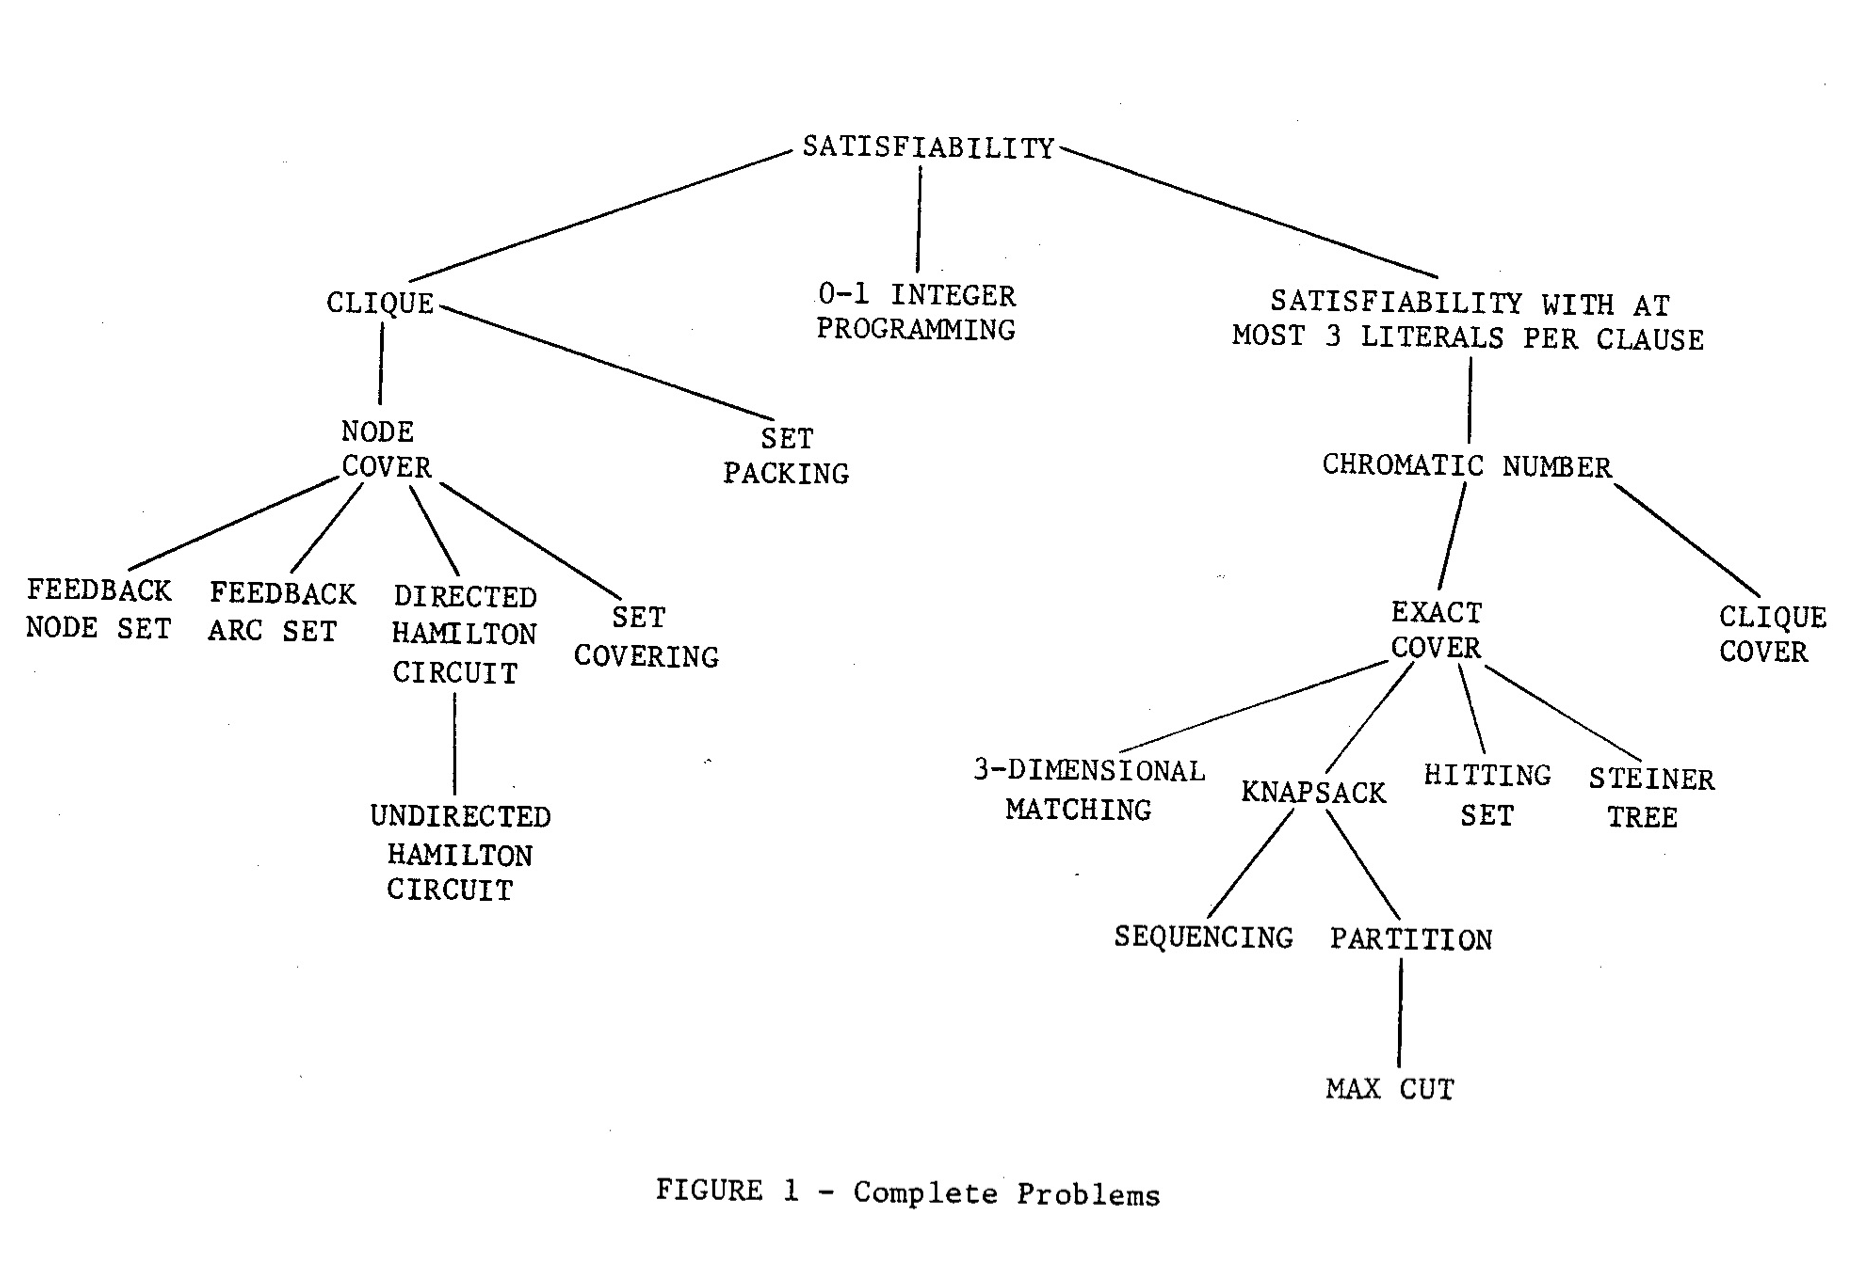
\includegraphics[width=1\textwidth]{images/Karp.png}
        \caption{Karp's 21 Problems}
    \end{figure}
\end{frame}
